\documentclass[conference]{IEEEtran}
\IEEEoverridecommandlockouts
% The preceding line is only needed to identify funding in the first footnote. If that is unneeded, please comment it out.
\usepackage{stfloats}
\usepackage{float}
\usepackage{cite}
\usepackage{amsmath,amssymb,amsfonts}
\usepackage{algorithmic}
\usepackage{graphicx}
\usepackage{textcomp}
\usepackage{xcolor}
\usepackage{booktabs}   % Para linhas de tabela profissionais
\usepackage{siunitx}    % Para o alinhamento decimal (coluna S)
\def\BibTeX{{\rm B\kern-.05em{\sc i\kern-.025em b}\kern-.08em
    T\kern-.1667em\lower.7ex\hbox{E}\kern-.125emX}}
\begin{document}
% Comando para criar cabeçalhos de tabela com quebra de linha
\newcommand{\thead}[1]{\begin{tabular}{@{}c@{}}#1\end{tabular}}

\title{Exploração de métricas cardíacas e componentes principais em diferentes estados de estresse\\
}

\author{\IEEEauthorblockN{1\textsuperscript{st} Anderson Nascimento}
\IEEEauthorblockA{\textit{Departamento de Teleinformática} \\
\textit{Universidade Federal do Ceará}\\
Fortaleza, Brasil \\
andersonmoura.cn@gmail.com}
\and
\IEEEauthorblockN{2\textsuperscript{rd} J. Rodrigo Nascimento}
\IEEEauthorblockA{\textit{Departamento de Teleinformática} \\
\textit{Universidade Federal do Ceará}\\
Fortaleza, Brasil \\
rodri.nasc@alu.ufc.br}
\and
\IEEEauthorblockN{3\textsuperscript{nd} Osvaldo Cavalcante Neto}
\IEEEauthorblockA{\textit{Departamento de Teleinformática} \\
\textit{Universidade Federal do Ceará}\\
Fortaleza, Brasil \\
osvaldomedeiros@alu.ufc.br}
\and
\IEEEauthorblockN{4\textsuperscript{th} Vinícius Lira}
\IEEEauthorblockA{\textit{Departamento de Teleinformática} \\
\textit{Universidade Federal do Ceará}\\
Fortaleza, Brasil \\
viniciuslavorlira@gmail.com}
}

\maketitle

\begin{abstract}
Este trabalho realiza uma análise exploratória de dados de variabilidade da frequência cardíaca obtidos por eletrocardiograma, investigando a relação entre marcadores fisiológicos e níveis de estresse. Utilizou-se o dataset Heart Rate Prediction to Monitor Stress Level, com preditores nos domínios do tempo, frequência e não linearidade, além das variáveis alvo de frequência cardíaca e condição de estresse. A análise incluiu inspeção de qualidade, visualizações, correlações e seleção de variáveis com base em multicolinearidade e poder discriminativo. Foram observados padrões compatíveis com a fisiologia: redução de indicadores vagais de curto prazo e aumento relativo da banda de baixa frequência sob maior demanda. A análise de componentes principais sintetizou a variabilidade em eixos interpretáveis, revelando a ordenação das condições ao longo do espectro autonômico. Os resultados destacam o valor da análise exploratória para apoiar o pré-processamento e a seleção de variáveis em aplicações de monitoramento do estresse.
\end{abstract}

\begin{IEEEkeywords}
eletrocardiograma, estresse, EDA, variabilidade da frequência cardíaca, PCA
\end{IEEEkeywords}

\section{Introdução}
A sensação de estresse é definida como a reação natural do organismo humano a situações de perigo, ameaça ou medo. Essa ferramenta
do corpo é comum a todo humano e nos coloca em estado de alerta, provocando sintomas físicos ou emocionais, como dor de cabeça,
batimentos cardíacos acelerados, sensação de desgaste fisíco, etc. Além disso, o estresse e seus sintomas são comumente atrelados ao desenvolvimento de
doenças cardiovasculares e mentais, o que mostra a importância de encontrarmos formas de prever ou detectar esse tipo de reação
do corpo. 

Na literatura, a relação entre o estresse e alguns parâmetros fisiologicos atrelados ao HRV (Heart Rate Variability) já tem sido estudada, indicando que
as varíaveis HRV são afetadas diretamente pelo estresse \cite{b1}, com atividades que geram estresse ocupacional impactando diretamente na redução da variação de frequência
cardíaca \cite{b2}, o que leva a menor flexibilidade do sistema nervoso autônomo e maior predominância da atividade simpática, o que gera o sentimento de fadiga física e mental.

Atualmente, com o avanço das tecnologias de monitoramento cardíaco \cite{b3}, como sensores de baixo custo e "wearables" e o aumento na disponibilização de bases de dados reais colhidos de pacientes, torna-se possível
analisar e visualizar o comportamento do estresse e suas consequencias. A análise desses dados nos permite identificar padrões fisiológicos e compreender sinais característicos 
da sensação de estresse, nos permitindo a criação de ferramentas baseadas em aprendizado estatístico para detecção e prevenção de estresse, capazes de auxiliar na detecção precoce e na prevenção 
do estresse em contextos clínicos, ocupacionais e cotidianos.

Nesse cenário, a análise exploratória de dados (EDA) surge como uma ferramenta essencial para compreender os dados, avaliar sua qualidade e identificar relações iniciais entre variáveis fisiológicas e 
níveis de estresse. O dataset Heart Rate Prediction to Monitor Stress Level, fornecido pela plataforma de dados Kaggle surge nesse contexto como uma fonte de dados
de grande valor para investigação científica.

Portanto, esse artigo tem como intuito principal realizar uma análise exploratória de dados sobre o referido dataset, buscando compreender sua estrutura, 
avaliar a qualidade das variáveis e identificar possíveis correlações entre parâmetros fisiológicos e níveis de estresse.

\section{Metodologia}

\subsection{Coleta de Dados}

O presente estudo utilizou o conjunto de dados “\textit{Heart Rate Prediction to Monitor Stress Level}” (Shanawad, 2021), disponível na plataforma Kaggle. O dataset reúne atributos fisiológicos derivados de sinais de eletrocardiograma (ECG) obtidos em diferentes indivíduos sob distintas condições de estresse, com o objetivo de analisar a relação entre variabilidade da frequência cardíaca e níveis de estresse.

Os dados foram fornecidos em seis arquivos .csv, divididos em subconjuntos de treinamento e teste, organizados nos domínios do tempo, frequência e não linearidade, contendo variáveis como MEAN$\textunderscore$RR, RMSSD, LF/HF, SD1, Sampen, entre outras. O conjunto de treinamento, utilizado neste trabalho, apresenta $N = 369.289$ amostras e $D = 36$ variáveis preditoras, além de duas variáveis-alvo: HR (frequência cardíaca) e condition (nível de estresse).

A variável condition possui L = 3 classes, distribuídas em no stress ($54,18\%$ das amostras), interruption ($28,47\%$ das amostras) e time pressure ($17,35\%$ das amostras), indicando leve desbalanceamento entre categorias. A análise descritiva inicial foi conduzida em {\tt Python} com a biblioteca Pandas, permitindo identificar dimensões, distribuição de classes e consistência dos dados. Apenas o conjunto de treinamento foi utilizado, visto que os arquivos de teste não contêm a variável HR, inviabilizando validação supervisionada. Dessa forma, todas as análises exploratórias e procedimentos de pré-processamento foram conduzidos exclusivamente sobre o conjunto de treinamento, abrangendo os três domínios de características.

\subsection{Análise Exploratória dos Dados}

O objetivo principal da análise exploratória é compreender a estrutura interna dos dados e identificar as variáveis mais pertinentes, ou seja, quais características fisiológicas possuem maior poder discriminatório para diferenciar os três estados de estresse definidos no estudo: no stress, interruption e time pressure. Além disso, por meio da análise, é possível detectar eventuais problemas, como a redundância, antes de se proceder à modelagem. Esta etapa é crucial para garantir a robustez das etapas futuras.\\

\noindent \textbf{Visualização dos Dados}\\

Para compreender a distribuição dos preditores, cada variável foi analisada individualmente, com suas estatísticas descritivas fundamentais: a média, o desvio padrão e a assimetria calculadas. As Tabelas \ref{tab:estatisticas_part1of3}, \ref{tab:estatisticas_part2of3} e \ref{tab:estatisticas_part3of3} apresentam essas estatísticas para cada preditor do conjunto de dados, permitindo identificar a magnitude e a dispersão de cada variável fisiológica. A análise foi realizada inicialmente de maneira incondicional, ou seja, sobre o conjunto de dados completo e, posteriormente, de modo condicional, levando em consideração as classes, visando avaliar o poder discriminatório de cada variável. Além disso, para cada uma das análises, foi  utilizado histogramas para visualizar a forma de cada distribuição e boxplots para identificar outliers. A Figura \ref{fig:HR} mostra o histograma e o box-plot incondicional da variável HR, que apresenta uma leve assimetria positiva e uma maior concentração dos dados entre 65-85 bpm. 

%IMAGENS E TABELAS

\begin{table*}[!b]
\centering
\caption{Estatísticas descritivas dos preditores (Parte 1 de 3).}
\sisetup{round-mode=places, round-precision=2}
\setlength{\tabcolsep}{0pt}
\begin{tabular*}{\textwidth}{@{\extracolsep{\fill}} l S[table-format=4.2] S[table-format=4.2] S[table-format=3.2] S[table-format=2.2] S[table-format=2.2] S[table-format=1.2] S[table-format=2.2] S[table-format=1.2] S[table-format=1.2] S[table-format=1.2] S[table-format=1.2] }
\toprule
\textbf{Estatística} & {MEAN\_RR} & {MEDIAN\_RR} & {SDRR} & {RMSSD} & {SDSD} & {SDRR\_RMSSD} & {HR} & {pNN25} & {pNN50} & {KURT} & {SKEW} \\
\midrule
Média           & 846.650104 & 841.965890 & 109.352531 & 14.977498 & 14.976767 & 7.396597 & 73.941824 & 9.841143 & 0.866001 & 0.523235 & 0.041628 \\
Desvio-padrão   & 124.603984 & 132.321005 & 77.117025 & 4.120766 & 4.120768 & 5.143834 & 10.337453 & 8.195574 & 0.990189 & 1.790348 & 0.699522 \\
Assimetria      & 0.648000 & 0.925513 & 2.363789 & 0.399529 & 0.399668 & 3.707939 & 0.411721 & 1.203114 & 1.264137 & 5.722209 & 1.223005 \\
\bottomrule
\end{tabular*}
\label{tab:estatisticas_part1of3}
\end{table*}

\begin{table*}[t]
\centering
\caption{Estatísticas descritivas dos preditores (Parte 2 de 3).}
\sisetup{round-mode=places, round-precision=2}
\setlength{\tabcolsep}{0pt}
\begin{tabular*}{\textwidth}{@{\extracolsep{\fill}} l S[table-format=1.2e-1] S[table-format=-1.2e-1] S[table-format=1.4] S[table-format=1.4] S[table-format=1.4] S[table-format=1.2] S[table-format=1.2] S[table-format=1.2] S[table-format=4.2] S[table-format=2.2] S[table-format=3.2] }
\toprule
\textbf{Estatística} & {\thead{MEAN\\\_REL\_RR}} & {\thead{MEDIAN\\\_REL\_RR}} & {\thead{SDRR\\\_REL\_RR}} & {\thead{RMSSD\\\_REL\_RR}} & {\thead{SDSD\\\_REL\_RR}} & {\thead{SDRR\_RMSSD\\\_REL\_RR}} & {\thead{KURT\\\_REL\_RR}} & {\thead{SKEW\\\_REL\_RR}} & {VLF} & {VLF\_PCT} & {LF} \\
\midrule
Média           & -0.000002 & -0.000465 & 0.018571 & 0.009701 & 0.009701 & 2.006817 & 0.523235 & 0.041628 & 2199.580170 & 64.289242 & 946.530252 \\
Desvio-padrão   & 0.000163 & 0.000868 & 0.005455 & 0.003897 & 0.003897 & 0.375845 & 1.790348 & 0.699522 & 1815.773422 & 16.774844 & 574.171780 \\
Assimetria      & 0.112796 & -0.948009 & 0.869543 & 1.258784 & 1.258784 & 0.838587 & 5.722209 & 1.223005 & 1.960735 & -0.410836 & 1.349076 \\
\bottomrule
\end{tabular*}
\label{tab:estatisticas_part2of3}
\end{table*}


\begin{table*}[t]
\centering
\caption{Estatísticas descritivas dos preditores (Parte 3 de 3).}
\sisetup{round-mode=places, round-precision=2}
\setlength{\tabcolsep}{0pt}
\begin{tabular*}{\textwidth}{@{\extracolsep{\fill}} l S[table-format=2.2] S[table-format=-1.2] S[table-format=2.2] S[table-format=1.2] S[table-format=1.2] S[table-format=4.2] S[table-format=3.2] S[table-format=1.2] S[table-format=2.2] S[table-format=3.2] S[table-format=-1.2] S[table-format=1.2] S[table-format=1.0] }
\toprule
\textbf{Estatística} & {LF\_PCT} & {LF\_NU} & {HF} & {HF\_PCT} & {HF\_NU} & {TP} & {LF\_HF} & {HF\_LF} & {SD1} & {SD2} & {sampen} & {higuci} & {datasetId} \\
\midrule
Média           & 34.095182 & 95.566718 & 39.245603 & 1.615576 & 4.433282 & 3185.356025 & 115.977200 & 0.048506 & 10.593708 & 154.178997 & 2.062471 & 1.182292 & 2.000000 \\
Desvio-padrão   & 16.040290 & 4.123365 & 45.398869 & 1.761073 & 4.123365 & 1923.227187 & 360.855129 & 0.049238 & 2.914795 & 109.170222 & 0.206999 & 0.062192 & 0.000000 \\
Assimetria      & 0.425164 & -1.645603 & 2.476530 & 2.021882 & 1.645603 & 1.452435 & 9.781091 & 2.159372 & 0.399668 & 2.363386 & -3.091012 & 0.335008 & 0.000000 \\
\bottomrule
\end{tabular*}
\label{tab:estatisticas_part3of3}
\end{table*}

\begin{figure*}[t]
\centerline{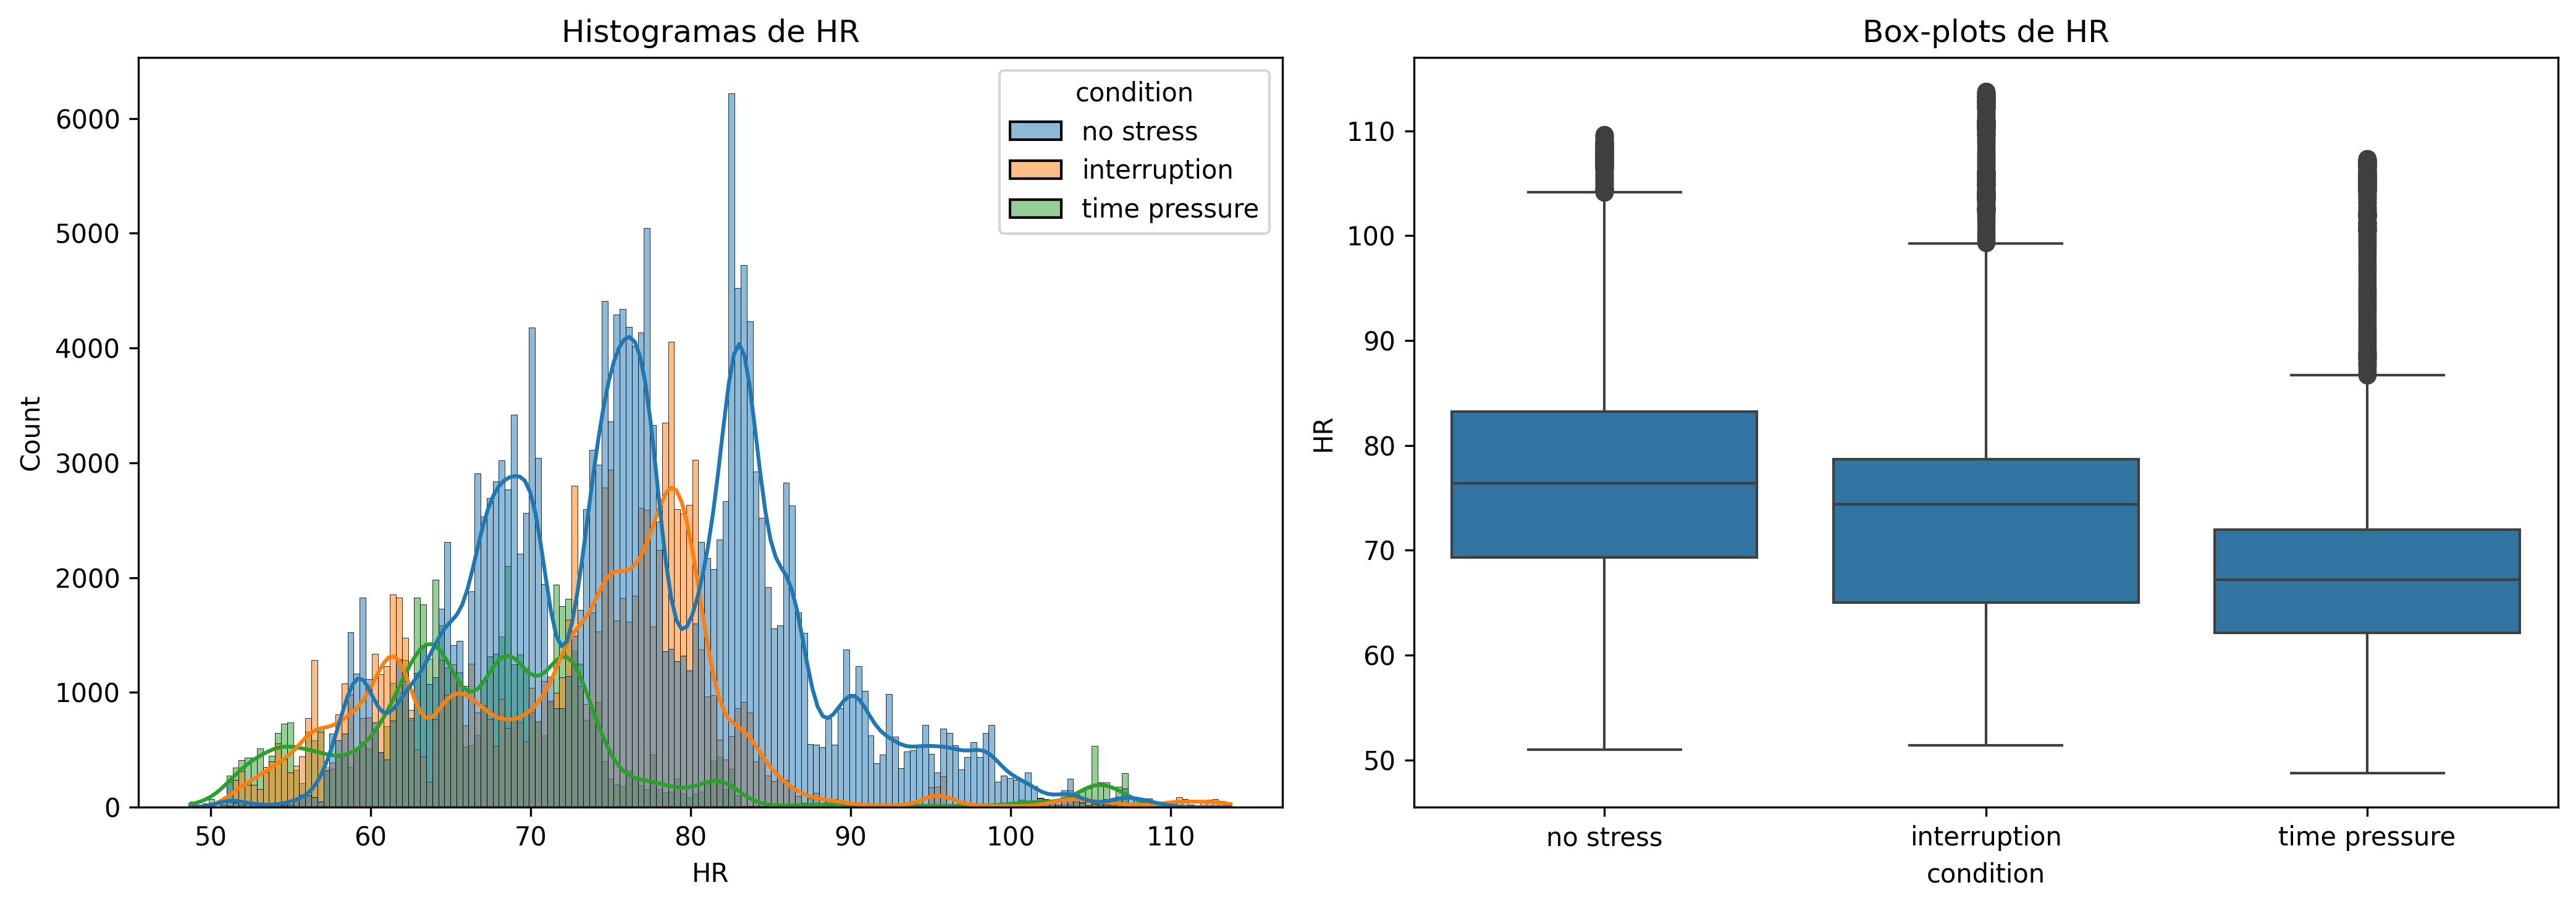
\includegraphics[width=0.7\linewidth]{imagens/HR.png}}
\caption{Histograma e box-plot incondicional de HR.}
\label{fig:HR}
\end{figure*}

\begin{figure}[htbp]
\centerline{\includegraphics[width=1\linewidth]{imagens/mean_RR.jpg}}
\caption{Histogramas de MEAN$\textunderscore$RR por classe.}
\label{fig:mean_RR}
\end{figure}


A Figura \ref{fig:mean_RR} apresenta os histogramas por classe de MEAN$\textunderscore$RR, que mostra claramente ser uma variável discriminatória, pois, dependendo da classe, temos diferentes distribuições.

A análise bivariada investigou as relações entre os pares de preditores utilizando diagramas de dispersão, com pontos coloridos conforme a classe \textit{condition}, permitindo avaliar visualmente a separação entre classes. Complementarmente, foi calculada uma matriz de correlação e visualizada como mapa de calor, facilitando a identificação de padrões de dependência linear e multicolinearidade entre os preditores.

\subsection{Refinação dos dados}
A fim de otimizar o conjunto de dados para a análise, foi realizada uma etapa rigorosa de seleção de características para remover preditores redundantes ou pouco informativos, utilizando dois critérios principais.

Para mitigar o problema de multicolinearidade entre os preditores, foi adotado um método heurístico baseado na matriz de correlação de Pearson, conforme proposto por Kuhn e Johnson \cite{b8}. O algoritmo remove o número mínimo de variáveis necessárias para que todas as correlações pareadas fiquem abaixo de um limiar, que foi definido para esse estudo como $0.8$. Em cada iteração, identifica-se o par mais correlacionado, calcula-se a média das correlações de cada variável e sugere-se a remoção daquela com maior média. O processo é repetido até que não restem correlações acima do limiar, reduzindo redundâncias e melhorando a estabilidade dos modelos preditivos. Para esse estudo, a variável HR não foi considerada na aplicação do algoritmo, devido ao seu uso como variável-alvo no futuro.

Em segundo lugar, foi realizada uma análise discriminante baseada nos resultados da análise univariada condicional. As variáveis que demonstraram baixo poder de separação entre as classes de estresse, ou seja, cujas distribuições se sobrepunham significativamente entre as diferentes condições, foram consideradas não informativas e também foram eliminadas.

Este processo de dupla filtragem resultou em um conjunto final e otimizado de preditores, que foi então utilizado para a subsequente Análise de Componentes Principais.

\subsection{Análise de Componentes Principais}

A Análise de Componentes Principais (PCA) é uma técnica estatística multivariada utilizada para a redução de dimensionalidade e extração de características. Sua principal importância reside na capacidade de transformar um conjunto complexo de variáveis correlacionadas em um novo conjunto, dimensionalmente menor, de variáveis não correlacionadas, chamadas componentes principais, retendo o máximo possível da variância original dos dados. A metodologia para a sua aplicação neste trabalho seguiu os seguintes passos propostos pela Dra. Michela Mulas\cite{b9}:

\begin{enumerate}
    \item \textbf{Padronização dos Dados:} O processo iniciou-se com centralização na média, onde a média de cada variável é subtraída de seus valores, e o escalonamento pela variância, onde o resultado é dividido pelo desvio padrão, de forma a  assegurar que a análise se concentrasse na estrutura de variância em detrimento da localização espacial dos dados.
    \item \textbf{Cálculo da Matriz de Covariância e Decomposição em Autovalores e Autovetores:} Com os dados padronizados, foi novamente calculada uma matriz de covariância. Ela foi então decomposta para encontrar seus autovalores ($\lambda$) e autovetores ($\vec{v}$). Nesta etapa, os autovetores representam as direções dos componentes principais, enquanto os autovalores correspondentes quantificam a magnitude da variância capturada por cada autovetor.

    \item \textbf{Projeção:} Os autovetores foram, então, ordenados de forma decrescente com base em seus autovalores, com os dados sendo projetados nos dois componentes principais com os maiores autovalores (PC1 e PC2).
\end{enumerate}

\section{Resultados}
\subsection{Estrutura dos dados e checagens iniciais}

Durante o preprocessamento, verificamos que os dados não continham valores ausentes, mas uma presença considerável de outliers. Os intervalos e valores observados para as variáveis estavam dentro do esperado fisiologicamente. A frequência cardíaca variou aproximadamente dentro da faixa adulta típica (cerca de 50–180 bpm entre os indivíduos), com médias em torno de valores normais em repouso ($\approx$ 60-80 bpm) e elevações compatíveis com situações de maior demanda experimental.

A presença do atributo condition permitiu comparar os grupos, mas as médias não seguiram o padrão fisiológico clássico (HR maior e HRV menor em estresse), indicando que as classes representam indivíduos diferentes e não medições repetidas. Ainda assim, a Figura \ref{fig:kdrhr_rmssd} evidencia o comportamento global das variáveis entre condições.

\begin{figure}[htbp]
    \centering
    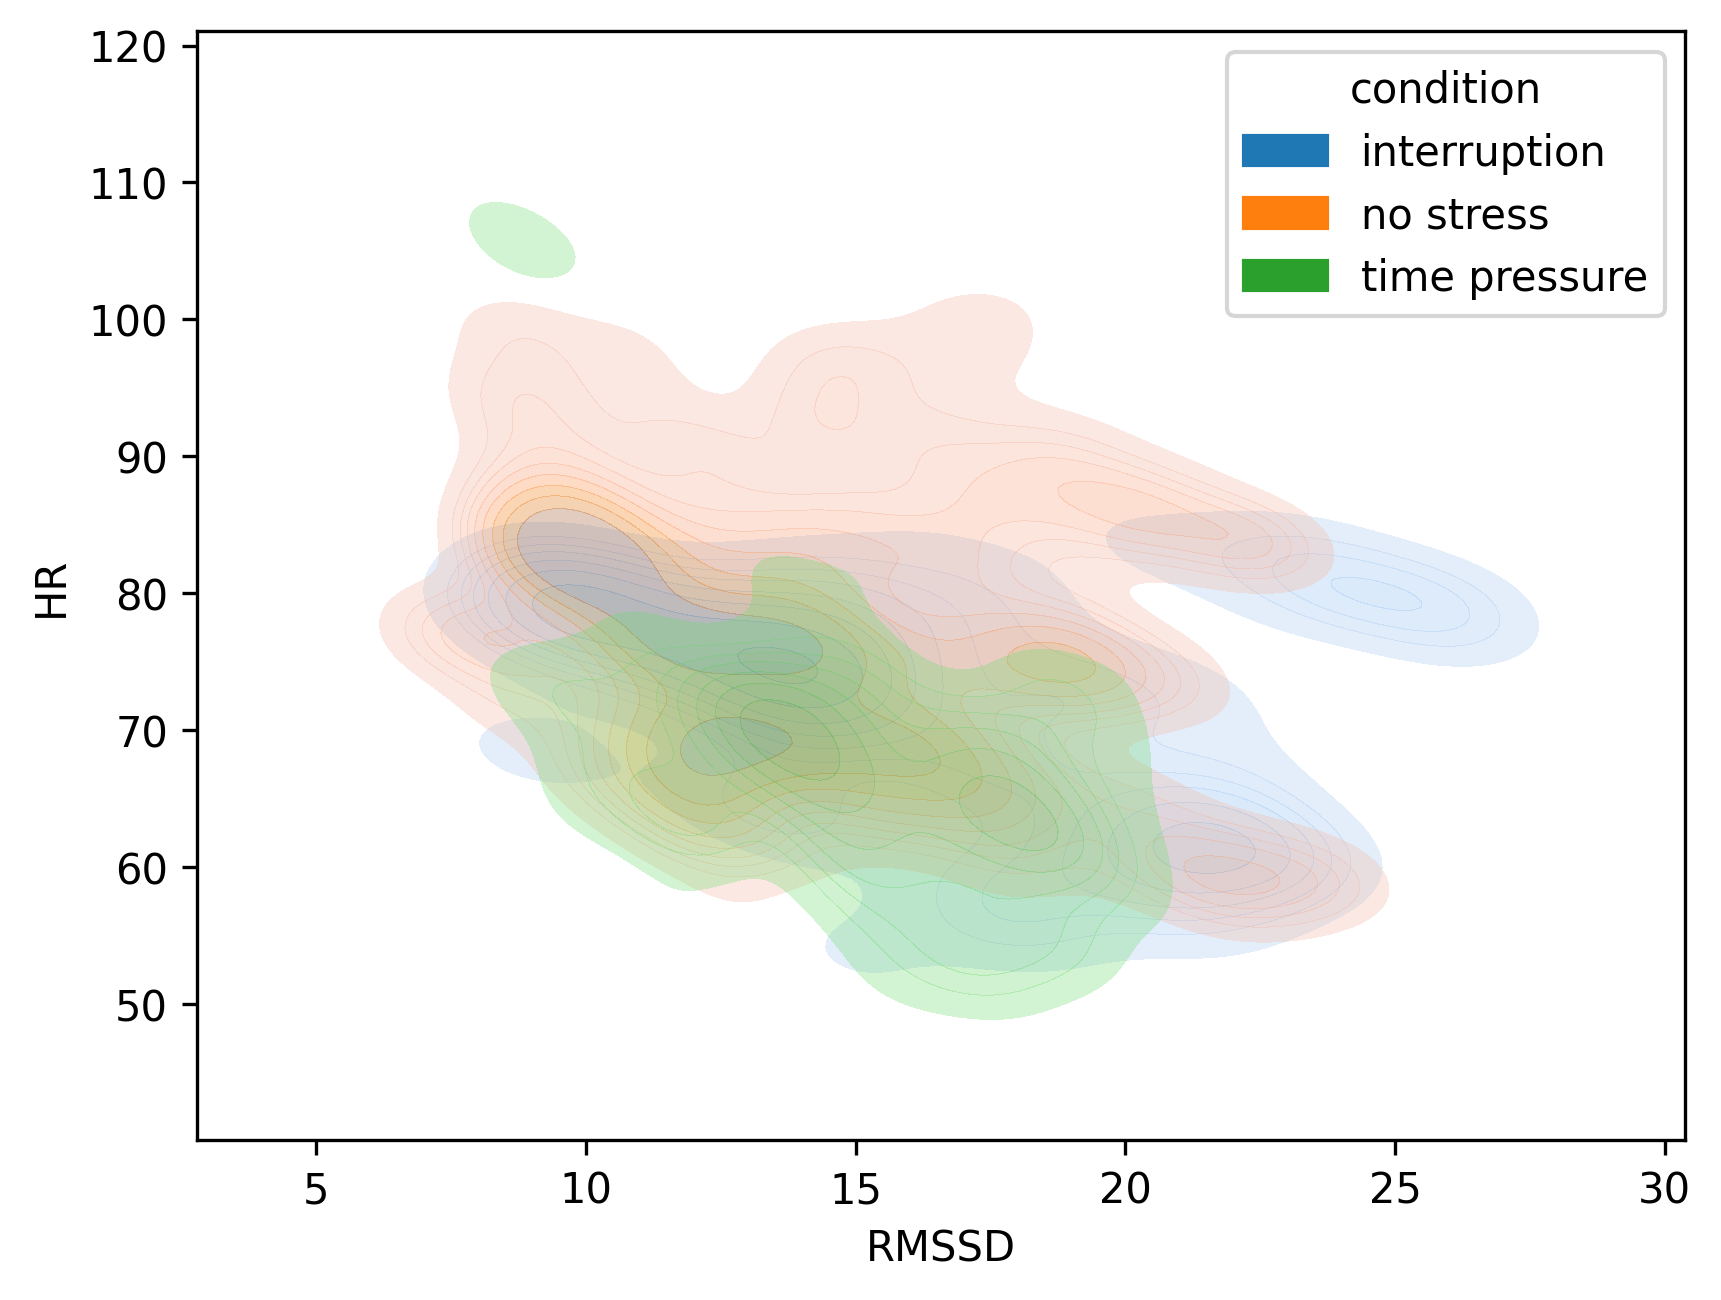
\includegraphics[width=0.7\linewidth]{imagens/kde_hr_rmssd_condition.png}
    \caption{Densidade bivariada HR × RMSSD nas diferentes condições.}
    \label{fig:kdrhr_rmssd}
\end{figure}

\subsection{Achados principais}

Após o pré-processamento e análise exploratória dos dados, identificamos padrões que relacionam as métricas de variabilidade da frequência cardíaca (HRV) com a frequência cardíaca medida (HR).

\subsubsection{Relação entre MEAN\_RR, MEDIAN\_RR e HR}

Inicialmente, há uma correlação inversa entre o intervalo R-R médio (MEAN\_RR) e a frequência cardíaca (HR), indicando que intervalos menores entre batimentos estão associados a HR mais alta. O que é esperado, pois quanto menor o RR, maior o número de batimentos por minuto \cite{R1}.

Em repouso o RR costuma ser $\approx1$ segundo (HR $\approx60$ bpm), enquanto RR de 0,5 s implica HR $\approx120$ bpm (taquicardia). Em que, considera-se taquicardia um ritmo cardíaco de repouso acima de 100 bpm \cite{R2}, valor este que de fato foi ultrapassado em alguns registros do conjunto de dados, sugerindo episódios de estresse ou esforço significativos.

\begin{figure}[htbp]
    \centering
    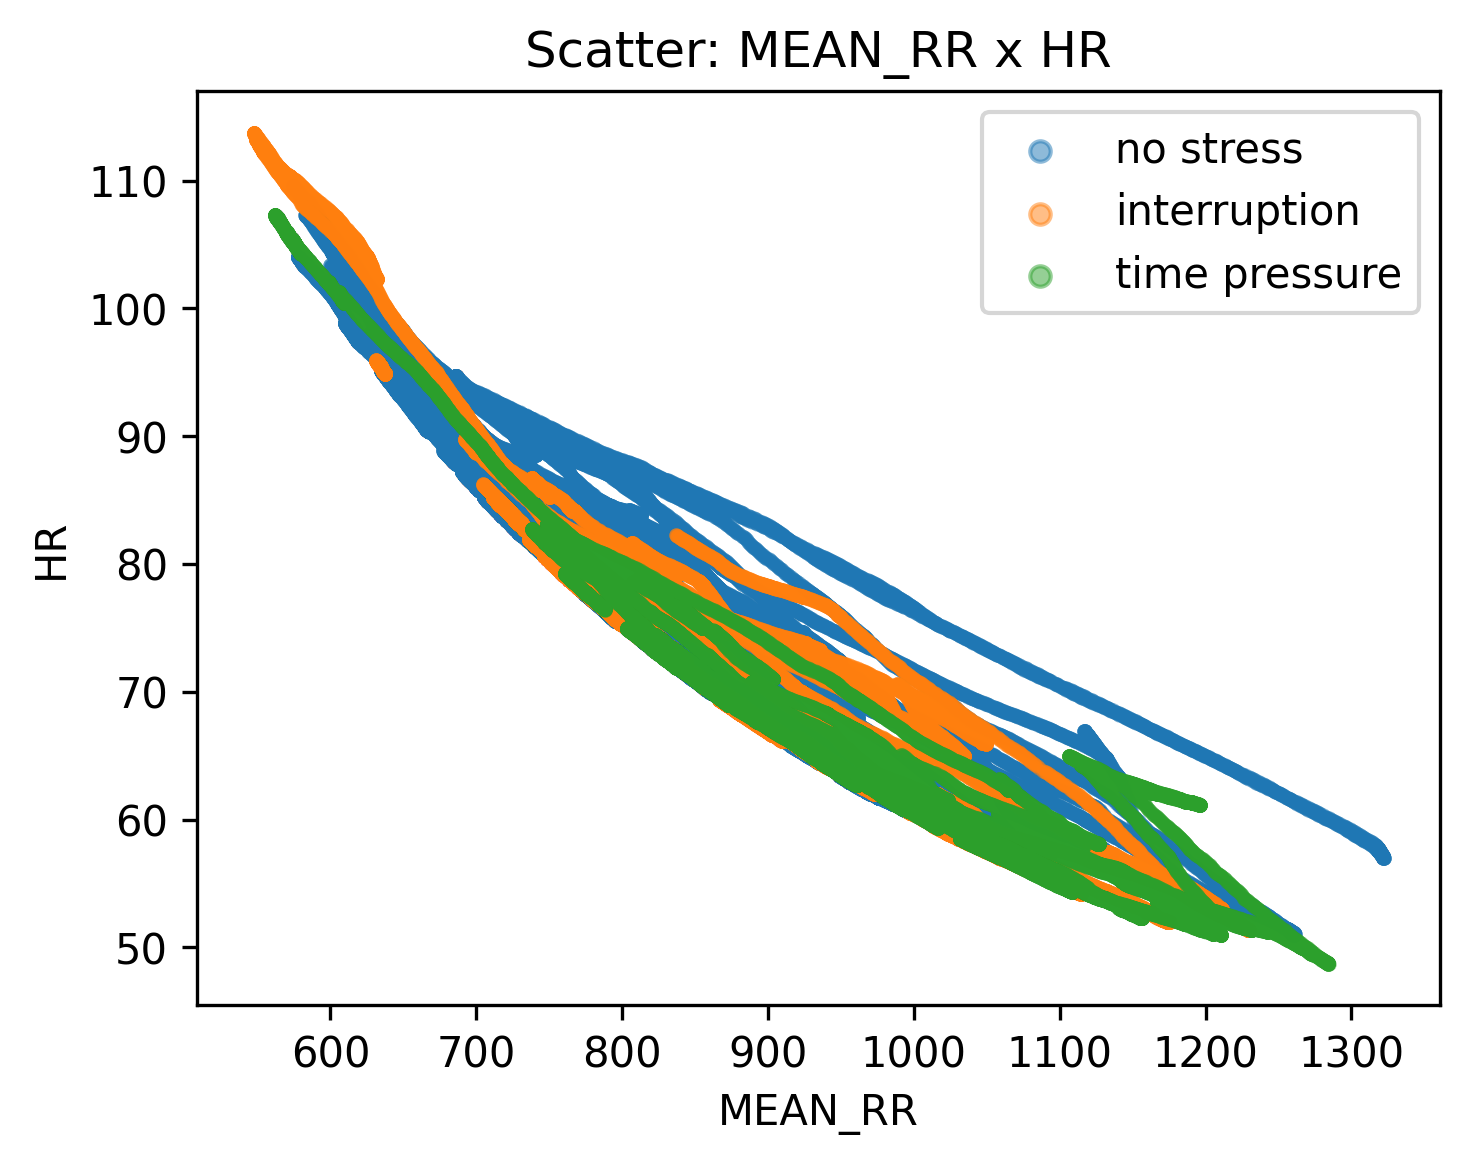
\includegraphics[width=0.7\linewidth]{imagens/Scatter MEAN_RR x HR.png}
    \caption{Dispersão HR × MEAN\_RR por classe}
    \label{fig:hrmedian_rr}
\end{figure}

A mesma correlação forte e negativa ocorre entre MEDIAN\_RR e HR ($r\approx -0,93$). O que é esperado por definição, já que MEDIAN\_RR e MEAN\_RR carregam essencialmente a mesma informação fisiológica da frequência cardíaca, sendo altamente correlacionados.

\begin{figure}[htbp]
    \centering
    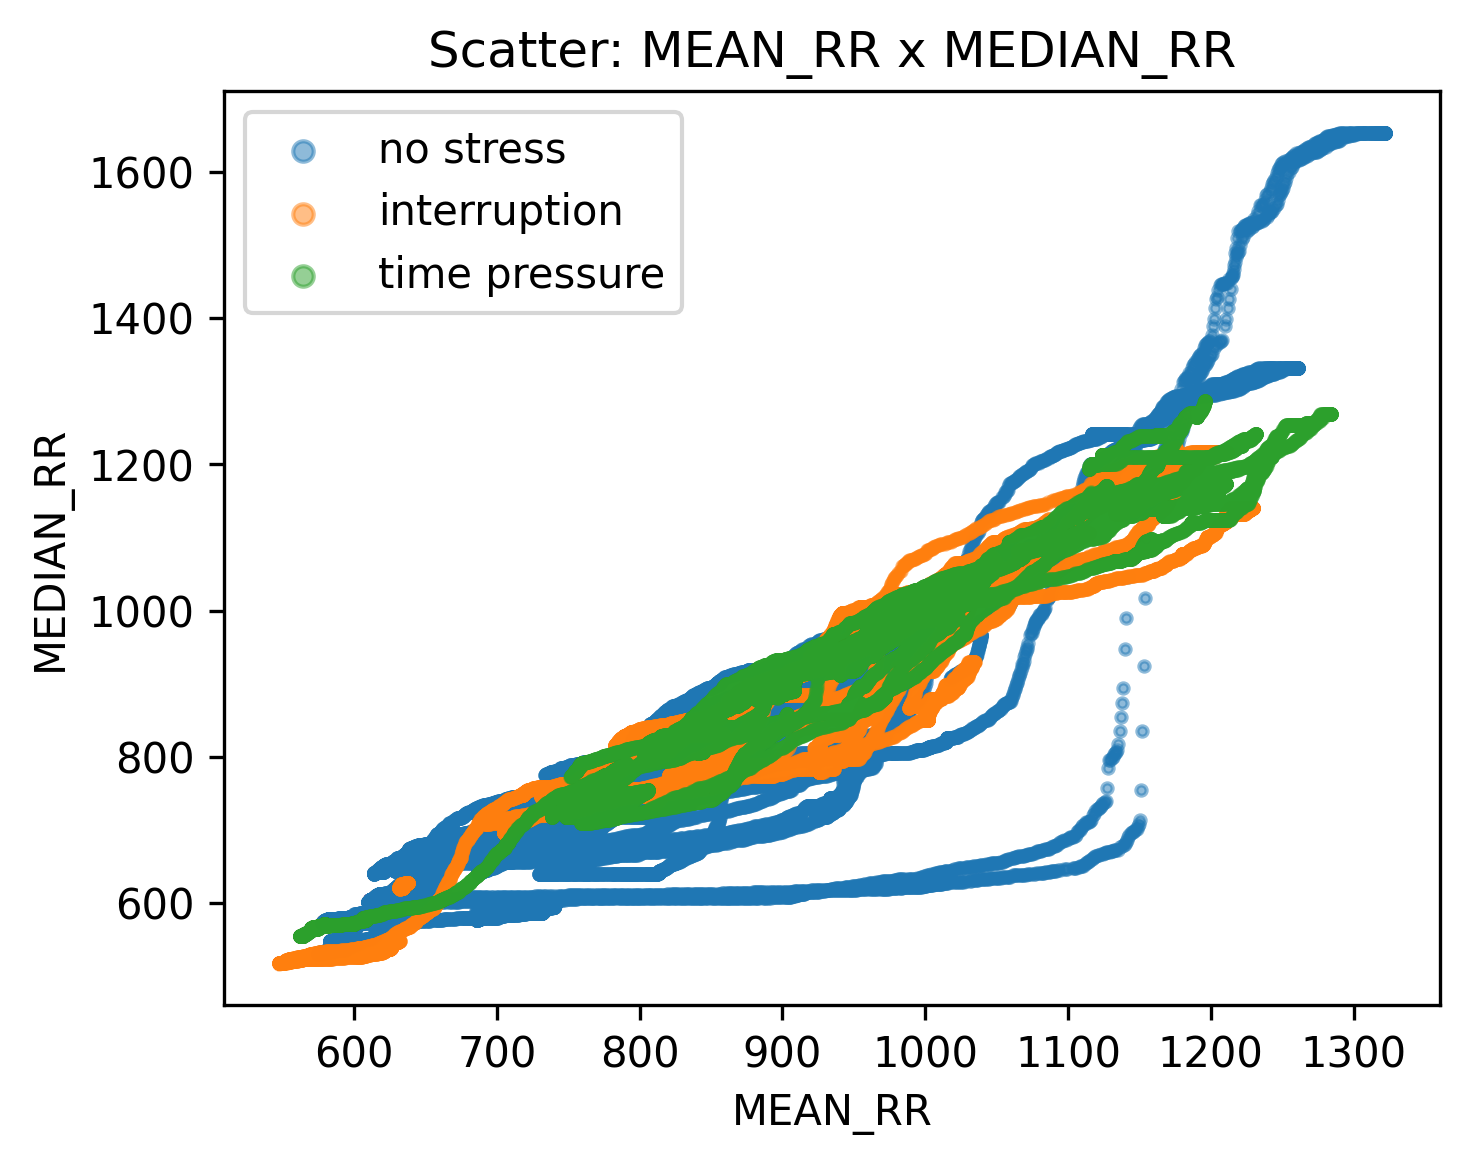
\includegraphics[width=0.8\linewidth]{imagens/Scatter MEAN_RR x MEDIAN_RR.png}
    \caption{Dispersão MEAN\_RR × MEDIAN\_RR por classe}
    \label{fig:hrmedian_rr}
\end{figure}

\subsubsection{Variabilidade de curto e longo prazo}

Observamos que métricas clássicas de variabilidade, especialmente aquelas dominadas pelo tônus parassimpático, tendem a diminuir quando a frequência cardíaca está elevada. Por exemplo, indicadores como RMSSD (raiz quadrada da média dos quadrados das diferenças sucessivas de RR) e pNN50 (porcentagem de intervalos RR sucessivos que diferem em mais de 50ms) exibiram valores menores em casos de HR alto. O que sugerem menor variabilidade batimento a batimento durante episódios de frequência elevada, coincidindo com o esperado em situações de estresse ou ativação simpática.

Na literatura, condições de estresse psicológico costumam se associar a HRV reduzida, incluindo queda em métricas como pNN50 e potência de alta frequência (HF), indicando menor influência vagal, ao mesmo tempo em que a razão LF/HF se eleva \cite{R1}. Nossos dados seguem esse padrão geral: as condições associadas a maior demanda apresentaram pNN50 e RMSSD mais baixos e LF/HF mais altos, refletindo um desequilíbrio autonômico compatível com a ativação simpática. Essa combinação de menor variabilidade de curto prazo e aumento relativo das oscilações de longo prazo sugere menor flexibilidade autonômica sob estresse, em consonância com o descrito na literatura \cite{R1}.

\begin{figure}[H]
    \centering
    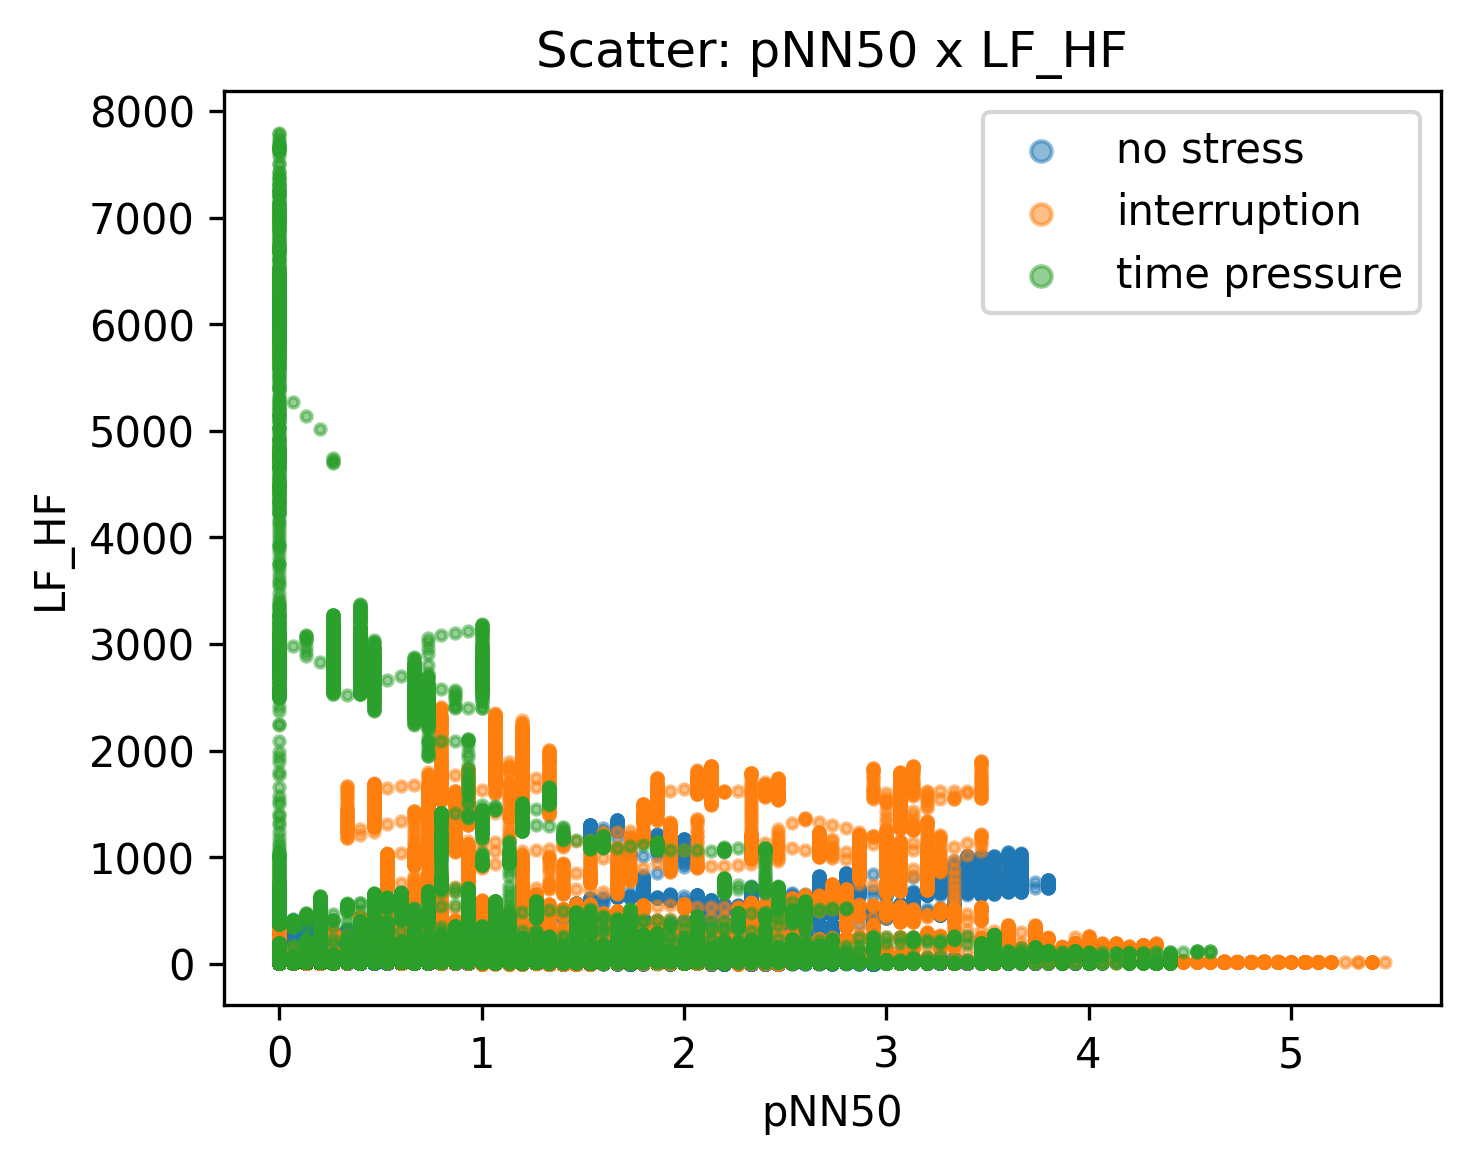
\includegraphics[width=0.8\linewidth]{imagens/Scatter pNN50 x LF_HF.png}
    \caption{Dispersão pNN50 × LF/HF por condição.}
    \label{fig:pnn50_X_LFHF}
\end{figure}

\subsubsection{Espectro e razão}

No domínio da frequência, vimos que, à medida que aumentava a demanda das tarefas (no stress $\rightarrow$ interruption $\rightarrow$ time pressure), a potência na banda de alta frequência (HF, 0,15–0,4 Hz) tendia a diminuir, enquanto a potência de baixa frequência (LF, 0,04–0,15 Hz) mostrava aumento relativo, resultando em elevação da razão LF/HF (Figura~\ref{fig:lfhf_box}). Esse comportamento indica uma redução da modulação vagal e maior predominância simpática, conforme descrito em estudos sobre respostas autonômicas ao estresse \cite{R1}.

As três condições do conjunto de dados apresentaram essa tendência de aumento progressivo da razão LF/HF, embora com grande dispersão. 

\begin{figure}[H]
    \centering
    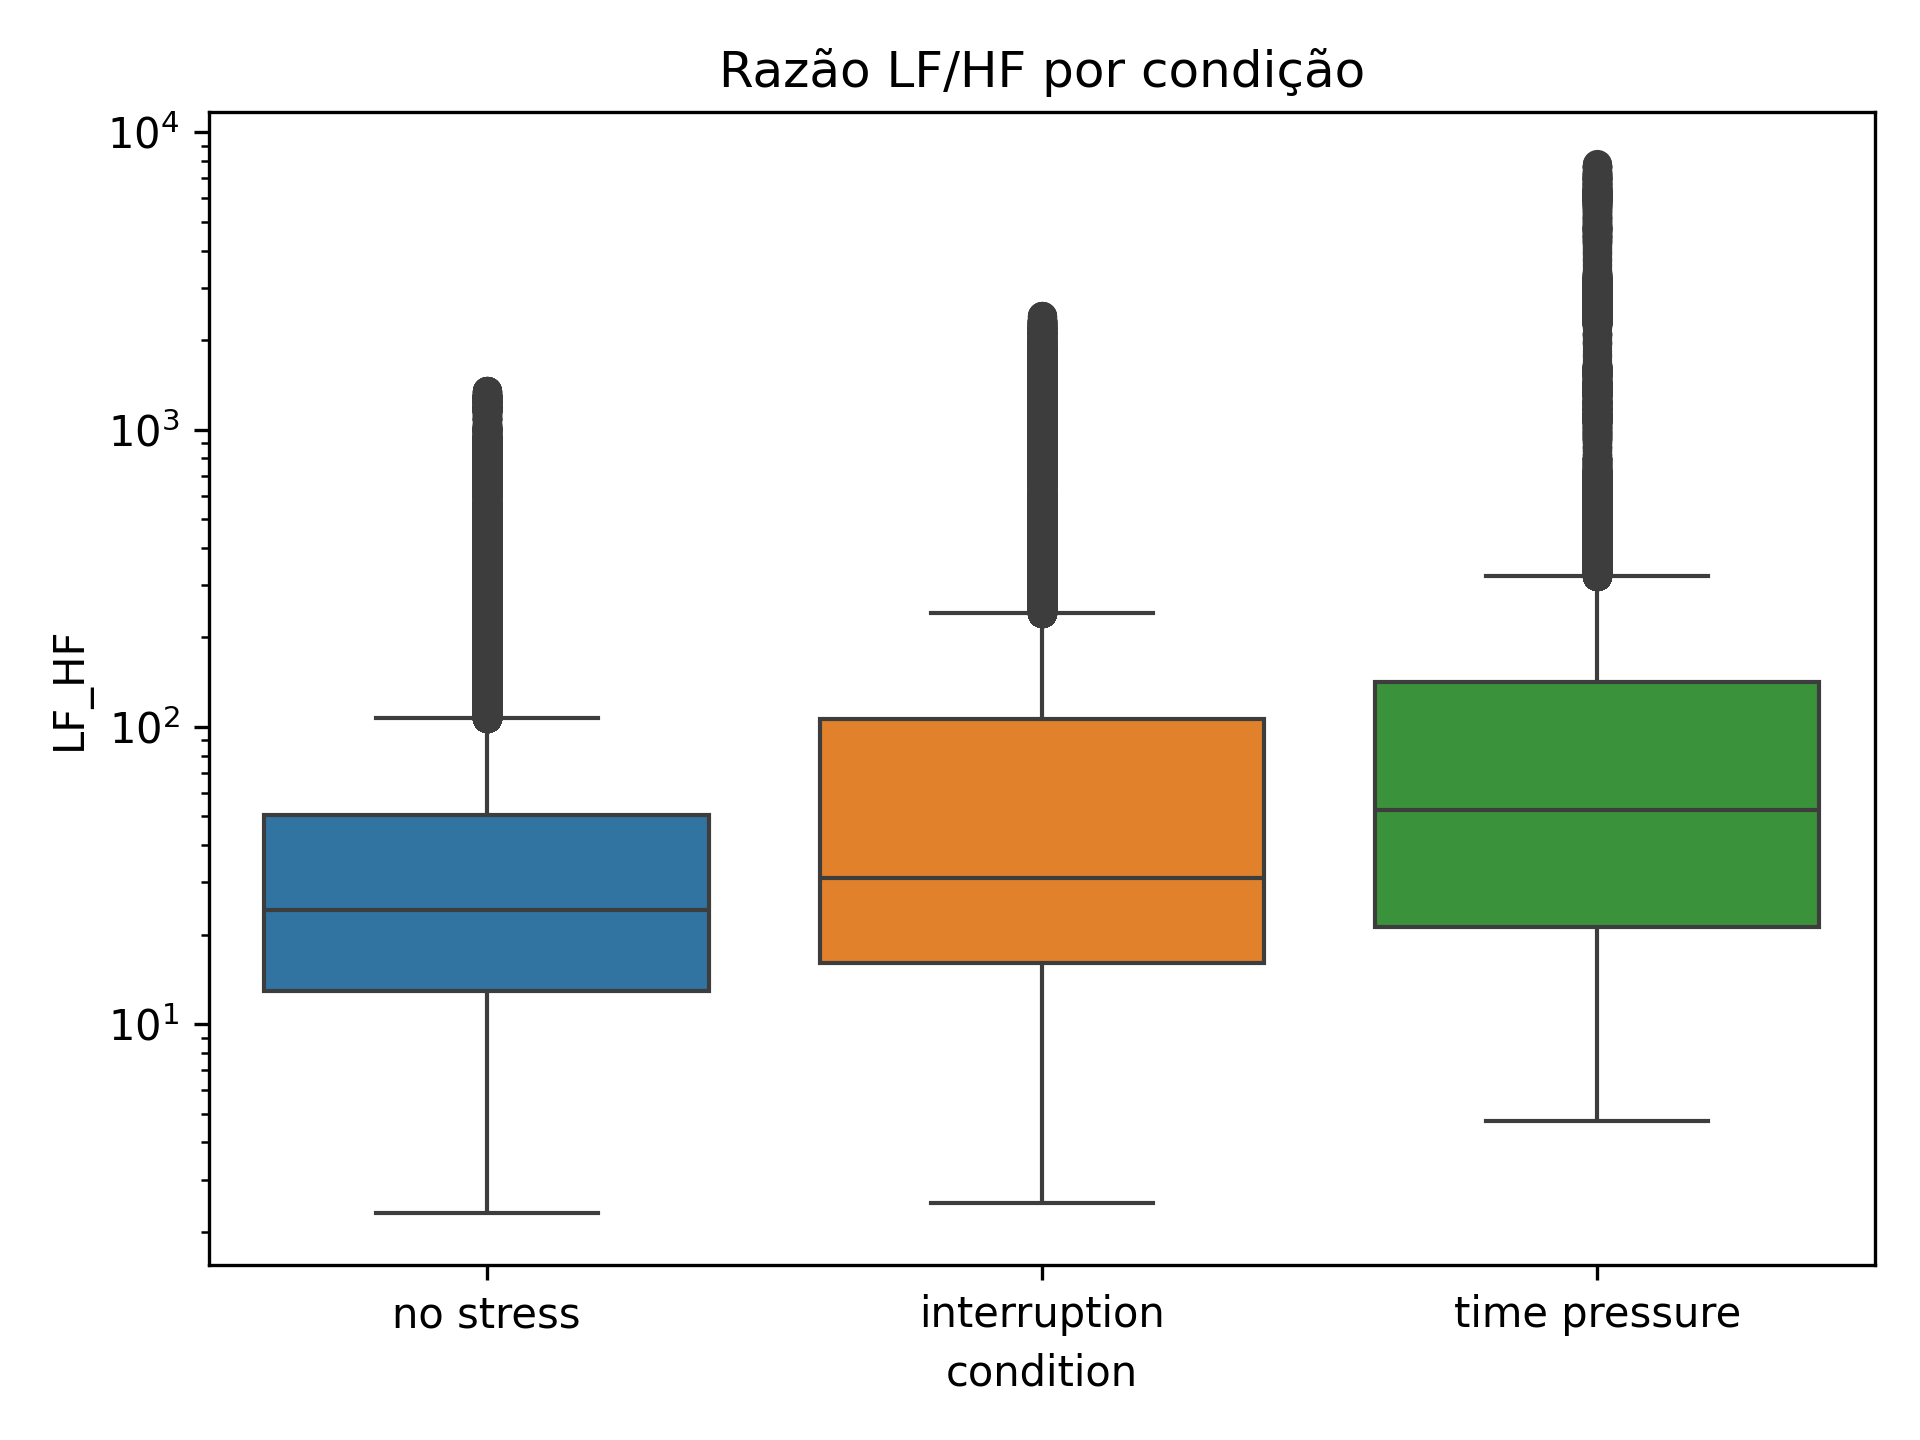
\includegraphics[width=0.8\linewidth]{imagens/box_lf_hf_condition.png}
    \caption{Boxplot LF/HF por condição.}
    \label{fig:lfhf_box}
\end{figure}

Quando a razão inversa (HF/LF) é observada, a interpretação se mantém invertida: em situações de maior demanda (menor influência vagal), HF diminui e LF aumenta, levando a LF/HF mais altos e, portanto, HF/LF mais baixos.

\begin{figure}[H]
    \centering
    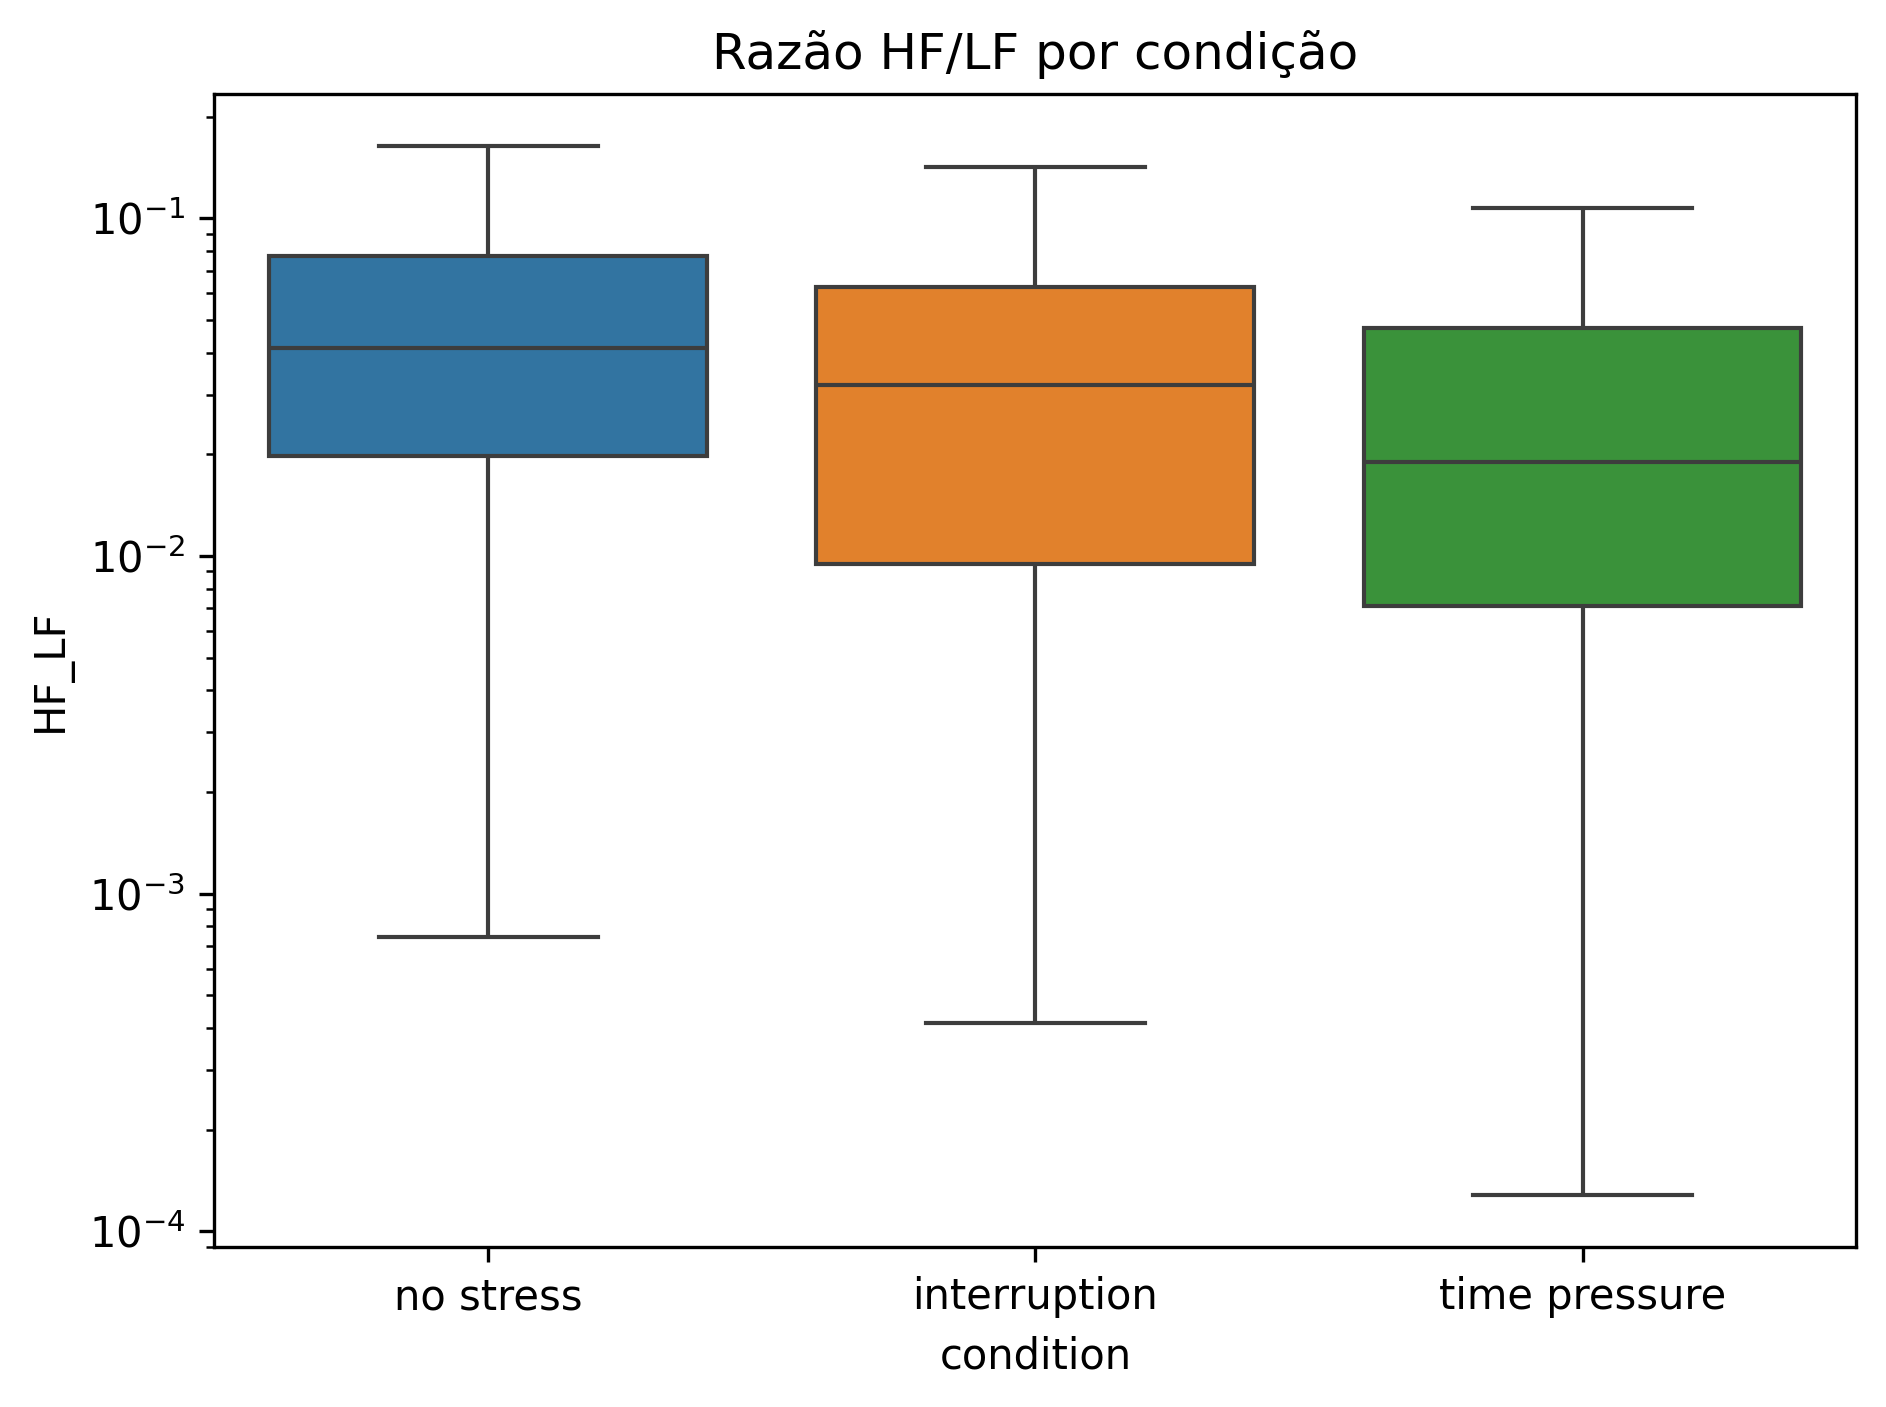
\includegraphics[width=0.8\linewidth]{imagens/box_hf_lf_condition_logscale.png}
    \caption{Boxplot HF/LF por condição.}
    \label{fig:lfhf_box}
\end{figure}

É importante lembrar que, embora HF represente predominantemente a atividade parassimpática e LF inclua componentes simpáticos e barorreflexos, a razão LF/HF deve ser interpretada com cautela, servindo apenas como indicador relativo de deslocamento do balanço autonômico.

\subsubsection*{4.4 Potência total e distribuição espectral}

Entre os índices de potência, a variável \textit{TP} (total power) representa a energia global da variabilidade dos intervalos RR, enquanto \textit{VLF\_PCT} descreve a contribuição relativa das oscilações de muito baixa frequência \cite{R3}. 

Na Figura~\ref{fig:BXP_TP_VLFPCT} observa-se que a potência total (\textit{TP}) apresentou valores ligeiramente mais altos sob \textit{time pressure}. 
Embora a literatura clássica reporte reduções de \textit{TP} e \textit{HF} em estresse agudo \cite{R1}, este comportamento divergente pode indicar particularidades do conjunto de dados e da segmentação dos sinais, não necessariamente uma inconsistência fisiológica. 

Assim como, \textit{VLF\_PCT} mostrou valores ligeiramente mais altos nessa condição, sugerindo maior participação relativa dos componentes de muito baixa frequência.

Essas variações, embora sutis, indicam que a resposta ao aumento de demanda não se limitou à redistribuição entre bandas (LF e HF), mas também envolveu alterações na potência total do espectro.

\begin{figure}[H]
    \centering
    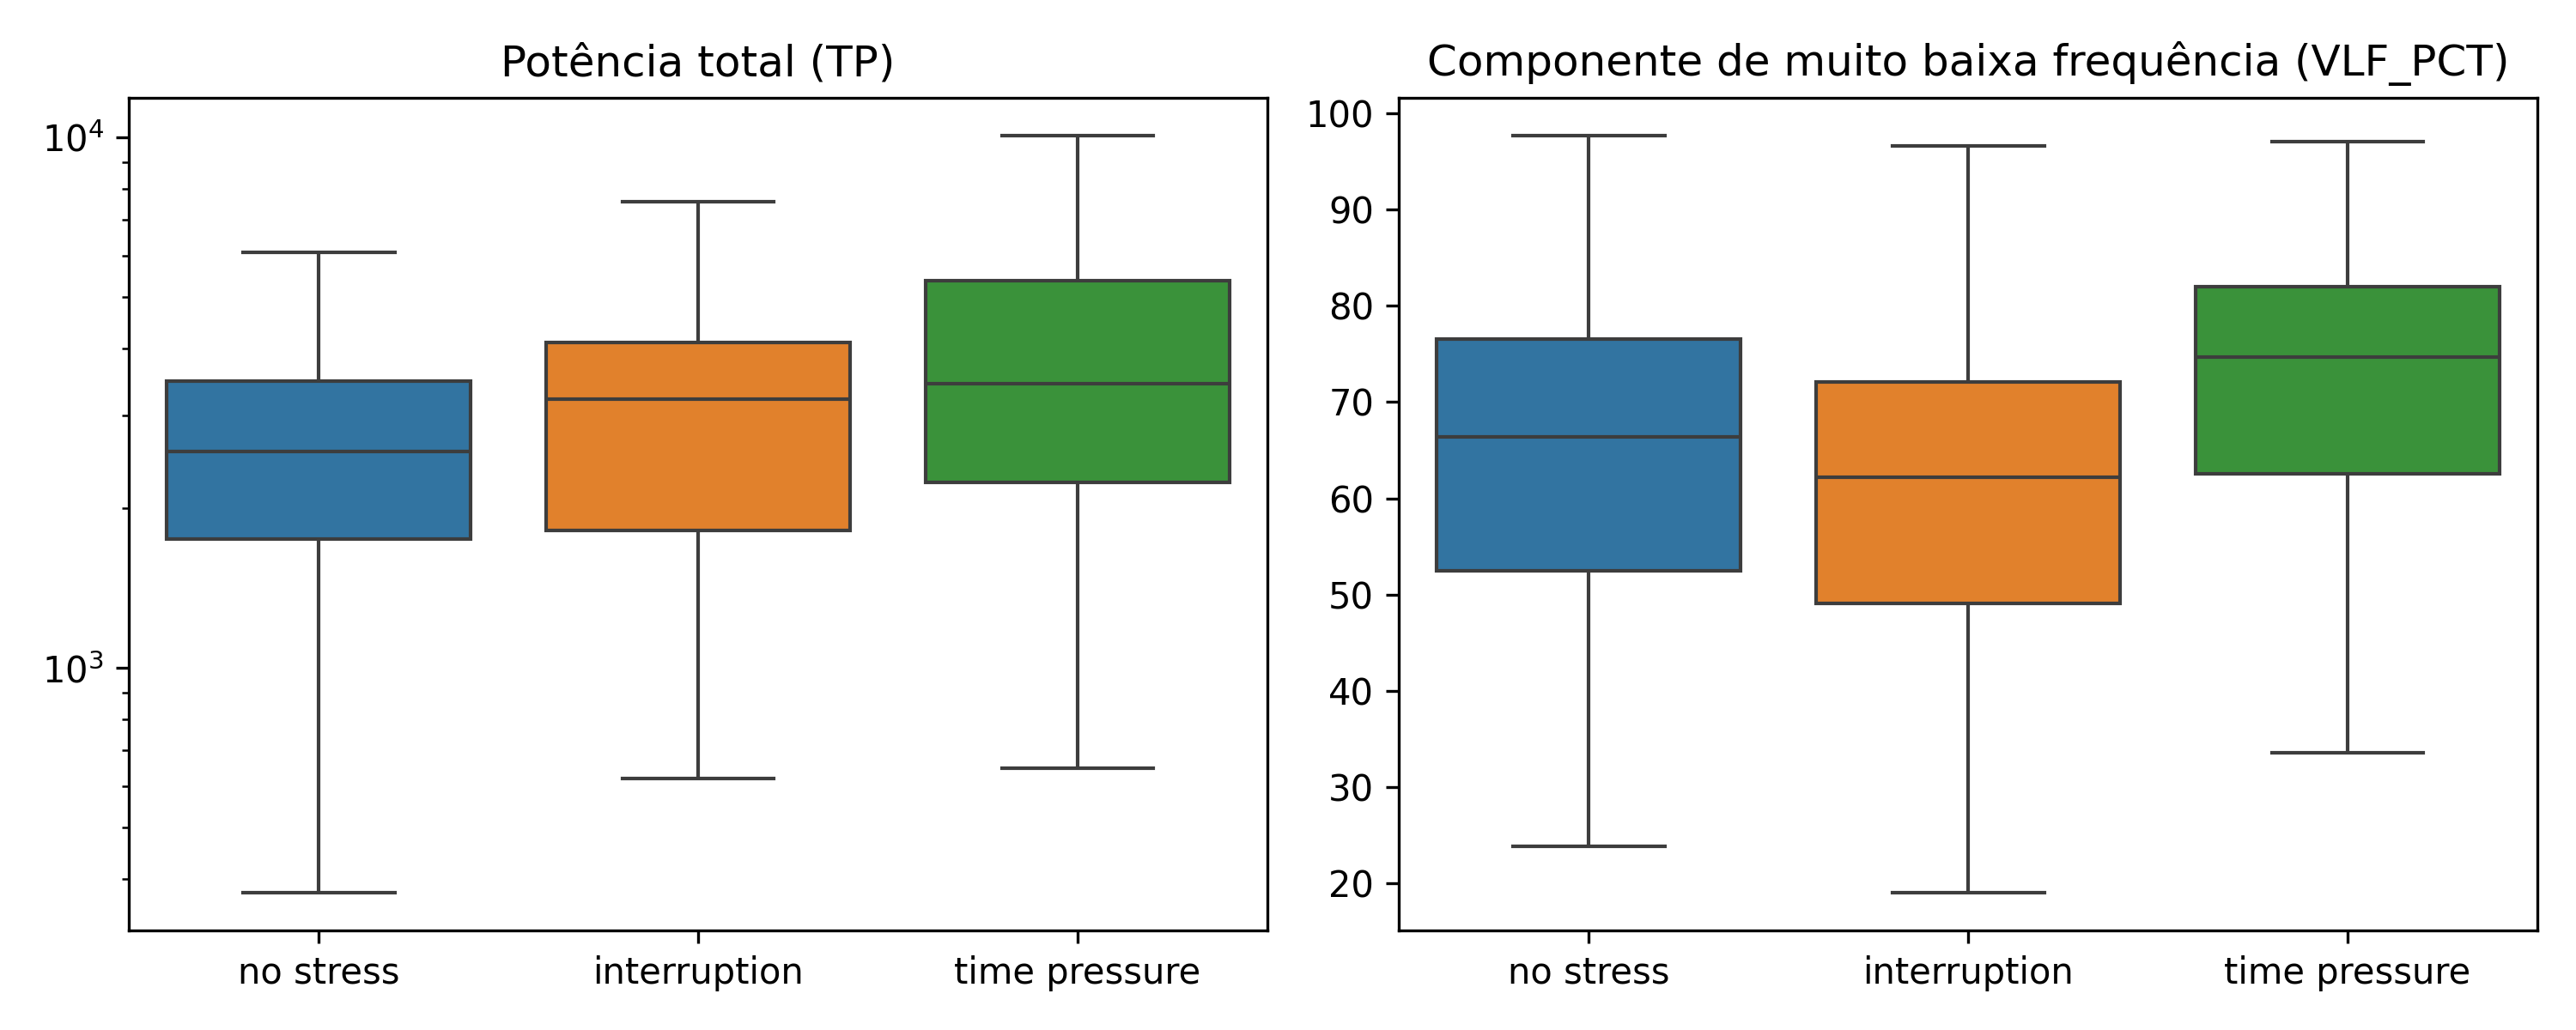
\includegraphics[width=\linewidth]{imagens/box_tp_vlfpct_condition.png}
    \caption{Boxplots por condição: \textit{TP}, \textit{VLF\_PCT}}
    \label{fig:BXP_TP_VLFPCT}
\end{figure}


\subsection{Redundância e seleção}

Vários dos preditores calculados apresentam definições semelhantes ou alto grau de correlação mútua. Por exemplo, RMSSD e pNN50 ambos quantificam variabilidade de curto prazo dominada pelo sistema parassimpático (vagal) e, como previsto, mostraram-se fortemente correlacionados entre si nos dados ($r \approx 0.79$). O que já era conhecido, tanto que RMSSD é frequentemente preferido ao pNN50 por ter propriedades estatísticas mais estáveis \cite{R3}. 

Essa redundância sugere que nem todos os preditores fornecem informação inédita para o modelo de regressão ou de classificação. Sabendo disso e das informações anteriores, escolhemos o subconjunto de preditores formado por 

(i) \textbf{Cronotropia} (\textit{HR}, \textit{MEDIAN\_RR}); 

(ii) \textbf{Variabilidade de curto prazo vagal} (\textit{RMSSD}, \textit{SDSD\_REL\_RR}); 

(iii) \textbf{Dispersão global de longo prazo} (\textit{SD2}, \textit{SDRR\_REL\_RR}); 

(iv) \textbf{Componentes espectrais} (\textit{LF}, \textit{HF}, \textit{VLF\_PCT}, \textit{TP}); e 

(v) a \textbf{Razão espectral inversa} (\textit{HF\_LF}).

Métricas não lineares, como a entropia amostral (Sampen), foram calculadas mas não mostraram poder discriminativo relevante.

\subsection{Análise de Componentes Principais (PCA) e Biplot}
O PCA aplicado aos 12 preditores padronizados explicou cerca de \textbf{71,2\%} da variância total nas duas primeiras componentes (\textit{PC1} = 40,5\%, \textit{PC2} = 30,7\%). 
O mapa \textit{PC1}$\times$\textit{PC2} exibiu sobreposição entre classes, mas com tendência ordenada: registros de \textit{time pressure} concentraram-se na região associada a \textit{HR} mais alta e \textit{MEDIAN\_RR} menor, enquanto \textit{no stress} ocupou o quadrante oposto, coerente com maior modulação vagal. 

A \textit{PC1} representou o eixo de controle cardíaco (com \textit{HR} e \textit{MEDIAN\_RR}), enquanto a \textit{PC2} refletiu diferenças de potência espectral (\textit{HF}, \textit{LF}, \textit{TP}). 
No \textit{biplot} (Figura~\ref{fig:biplot_pca}), as cargas (\textit{loadings}) reforçam essa separação: \textit{HR} e \textit{MEDIAN\_RR} mostram orientação oposta, confirmando correlação negativa, e as variáveis \textit{HF} e \textit{HF\_LF} agrupam-se, indicando captação conjunta do componente vagal.  

Em síntese, o \textit{biplot} evidencia um eixo principal associado à frequência cardíaca e outro à variação espectral, reproduzindo o padrão fisiológico esperado e mostrando que as condições se distribuem de forma contínua ao longo do espectro autonômico.

\begin{figure}[H]
    \centering
    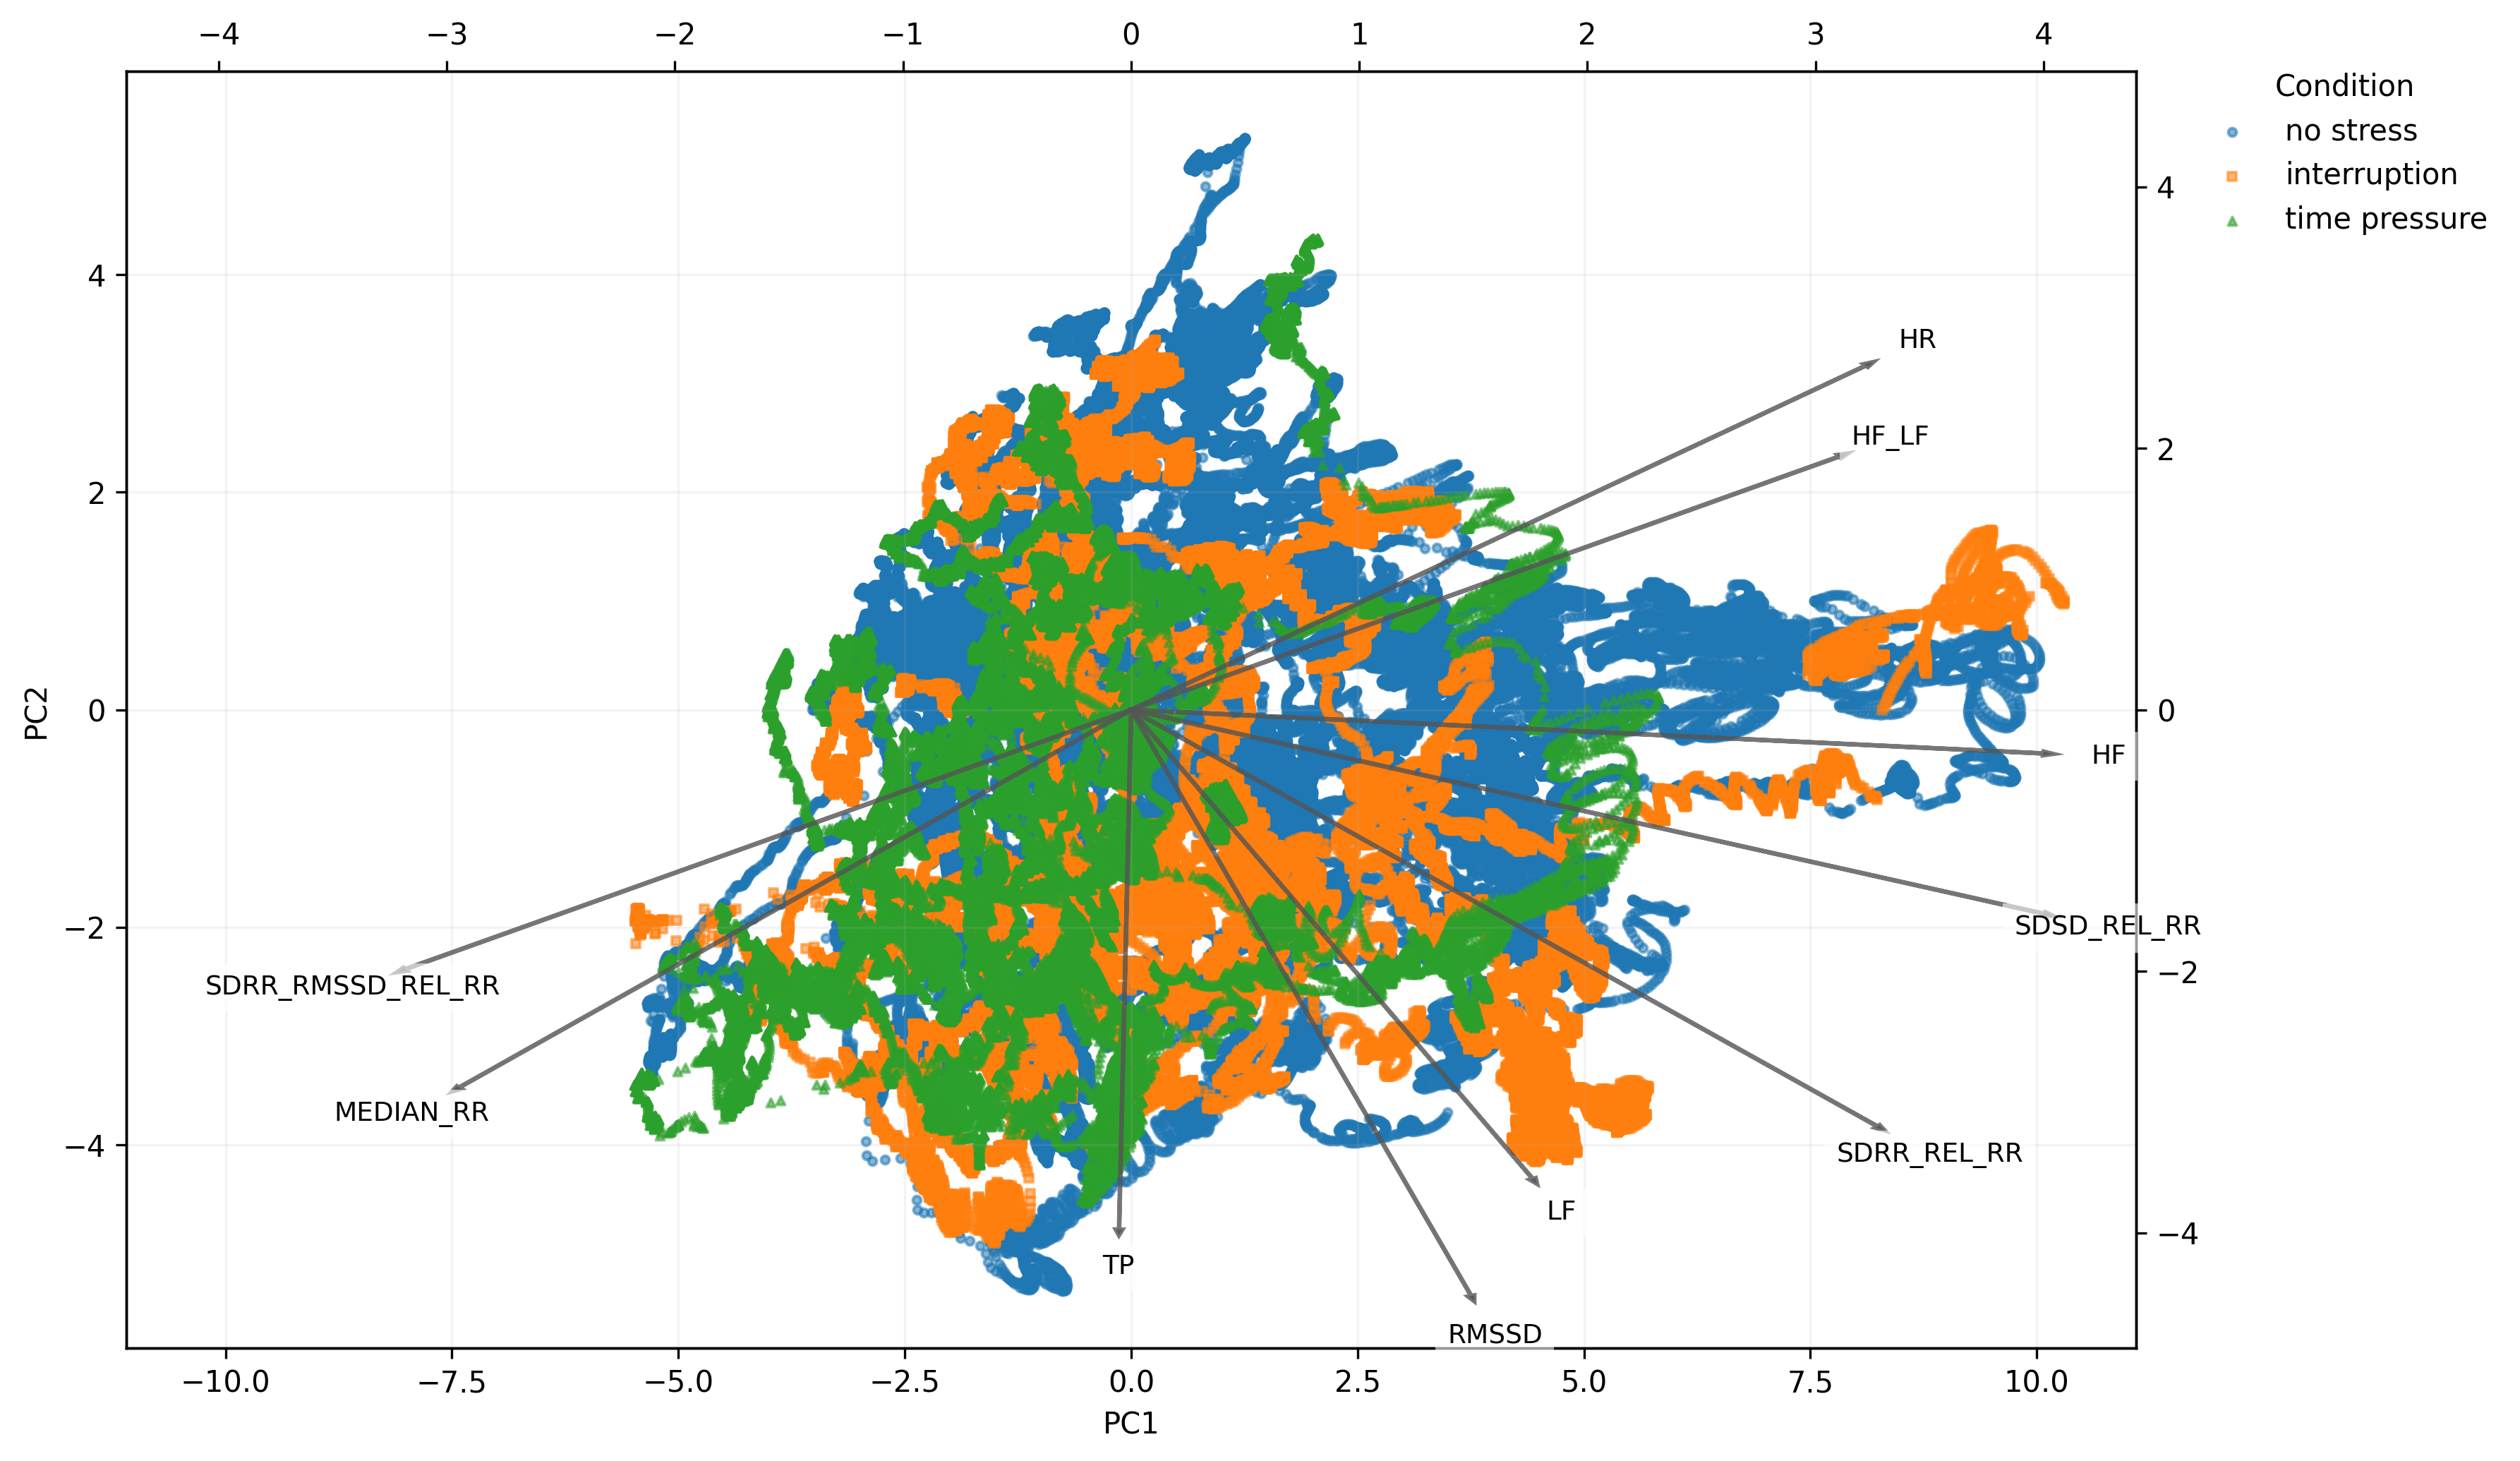
\includegraphics[width=\linewidth]{imagens/biplot_pca_2variaveis.png}
    \caption{Biplot das duas primeiras componentes principais (PC1 e PC2) obtidas a partir dos 12 preditores padronizados.}
    \label{fig:biplot_pca}
\end{figure}


\section{Conclusão}

Em conclusão, a explicação e discussão crítica dos resultados do pré-processamento reforçam que os dados estão consistentes com os princípios da fisiologia cardíaca. O pré-processamento, incluindo padronização e eliminação de variáveis altamente correlacionadas, preservou a diversidade fisiológica entre métricas cronotrópicas, temporais e espectrais. Dessa forma, conseguimos enriquecer a análise exploratória com contexto biológico, oferecendo ao leitor uma compreensão mais profunda de como os resultados do pré-processamento se conectam à realidade fisiológica subjacente aos dados.


\begin{thebibliography}{00}
\bibitem{b1} Kim HG, Cheon EJ, Bai DS, Lee YH, Koo BH. Stress and Heart Rate Variability: A Meta-Analysis and Review of the Literature. Psychiatry Investig. 2018 Mar;15(3):235-245. doi: 10.30773/pi.2017.08.17. Epub 2018 Feb 28. PMID: 29486547; PMCID: PMC5900369.
\bibitem{b2} Järvelin-Pasanen S, Sinikallio S, Tarvainen MP. Heart rate variability and occupational stress-systematic review. Ind Health. 2018 Nov 21;56(6):500-511. doi: 10.2486/indhealth.2017-0190. Epub 2018 Jun 16. PMID: 29910218; PMCID: PMC6258751.
\bibitem{b3} Salai, Mario, Vassányi, István, Kósa, István, Stress Detection Using Low Cost Heart Rate Sensors, Journal of Healthcare Engineering, 2016, 5136705, 13 pages, 2016. https://doi.org/10.1155/2016/5136705 
\bibitem{R1} R. Shaffer and J. P. Ginsberg, “An Overview of Heart Rate Variability Metrics and Norms,” Frontiers in Public Health, vol. 5, p. 258, Apr. 2017. [Online]. Available: https://pmc.ncbi.nlm.nih.gov/articles/PMC5900369/
\bibitem{R2} American Heart Association, “Tachycardia (Fast Heart Rate),” Heart.org, 2024. [Online]. Available: https://www.heart.org/en/health-topics/arrhythmia/about-arrhythmia/tachycardia--fast-heart-rate.
\bibitem{R3} Task Force of the European Society of Cardiology and the North American Society of Pacing and Electrophysiology, “Heart rate variability: Standards of measurement, physiological interpretation and clinical use,” Circulation, vol. 93, no. 5, pp. 1043–1065, 1996. [Online]. Available: https://www.escardio.org/static-file/Escardio/Guidelines/Scientific-Statements/guidelines-Heart-Rate-Variability-FT-1996.pdf
\bibitem{b8} Kuhn, M., \& Johnson, K. (2018). Applied predictive modeling. Springer.

\bibitem{b9} MULAS, M. Applied computational intelligence: Data pre-processing and principal component analysis. [S.l.: s.n.], 2025. 1 arquivo PDF. Aula da disciplina TI0175 – Applied Computational Intelligence, Universidade Federal do Ceará, 2025.
\end{thebibliography}


\end{document}
